\chapter{Rezultati}
V tem poglavju bom opisal rezultate, ki sem jih pridobil. Kot sem že omenil, bo večji del preizkušanja programa opravljen na slikah, kjer bodo nekateri piksli manjkali. Gre za problem, ki ga je moč lepo vizualizirati, saj pogosto pri surovih podatkih ni lahko definirati njihovo točnost, zaradi česar težko interpretiramo, kako koristen je sam algoritem.

Prav tako bom opisal točnost rezulatov različnih metod kot tudi čas izvajanja posameznih metod. Probleme bom zagnal tudi na različnih vrst podatkov, npr. podatkih ki so generirani normalno kot tudi enakomerno porazdeljeno.
Zaradi interpretacije, slike razdelimo v več skupin, za katere opišemo ugotovitve.

Vse slike si je mogoče v boljši kakovosti ogledati na povezavi \url{https://tinyurl.com/yb7cjdv7}. 

\section{Velika črno-bela slika}
Same teste algoritmov najprej poženemo na veliki, črno-beli sliki, velikosti $1000\times1000$ pikslov. Taka izbira je smiselna, iz vidika, da imamo dovolj podatkov, potrebnih za rekonstrukcijo. Ker je časovna zahtevnost algoritmov pri večjih slikah, kot bomo videli v nadaljevanju že precej velika, nam ta faza testiranja služi kot preverjanje delovanja samih algoritmov. Same podrobnosti razlik med rezultati si bomo zato podrobneje pogledali na manjših slikah v nadaljevanju. Algoritme preizkušamo trikrat, na podatkih z deleži znanih vrednosti $0.35, 0.45$ in $0.6$. \todo{Smiselna postavitev teskst-slik in velikosti}
\renewcommand{\mapa}{Poglavja/Slike/grayscale1000}

\begin{figure}[!ht]
    \centering
    \begin{subfigure}{0.49\linewidth}
        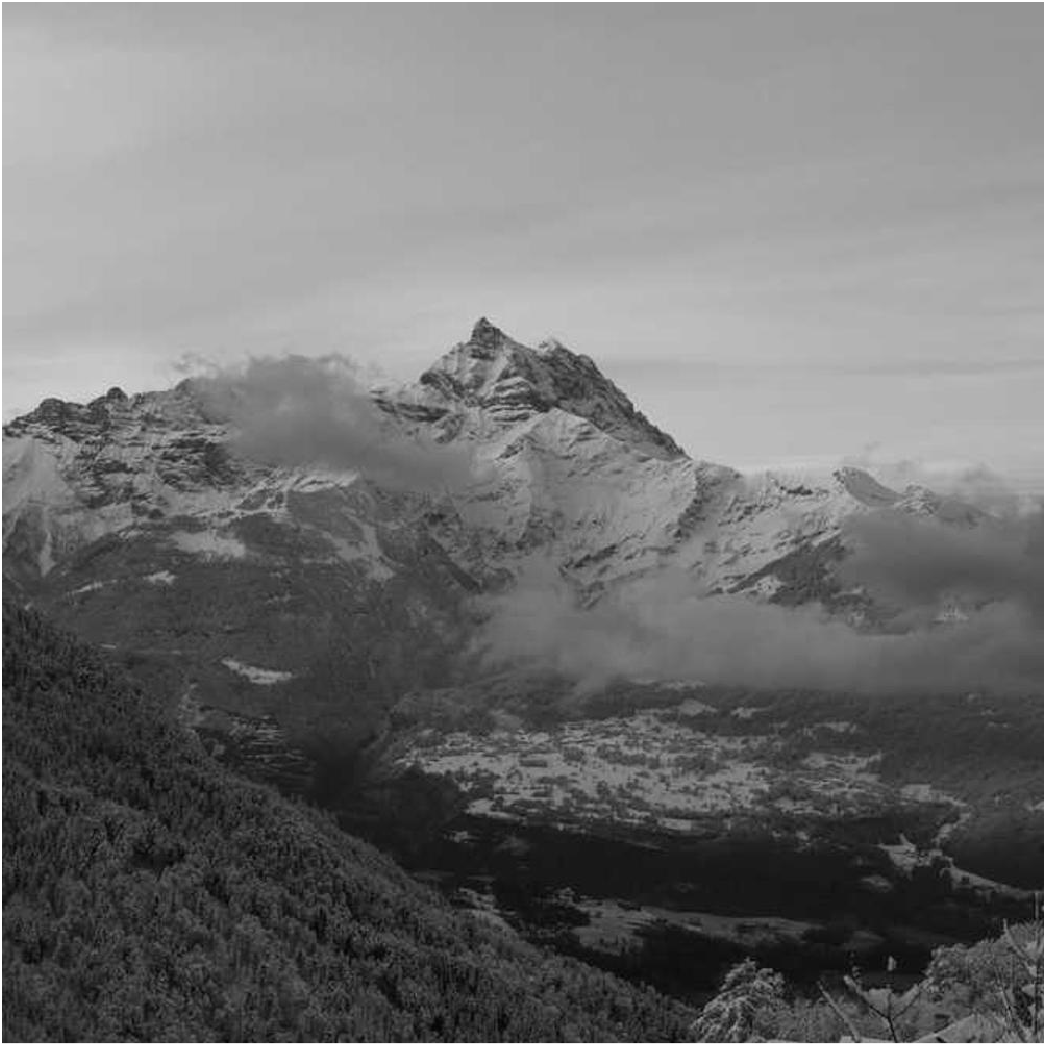
\includegraphics[width=\linewidth]{\mapa/slikaInput.png}
        \caption{Originalna slika.}
    \end{subfigure}
    \hfill
    \begin{subfigure}{0.49\linewidth}
        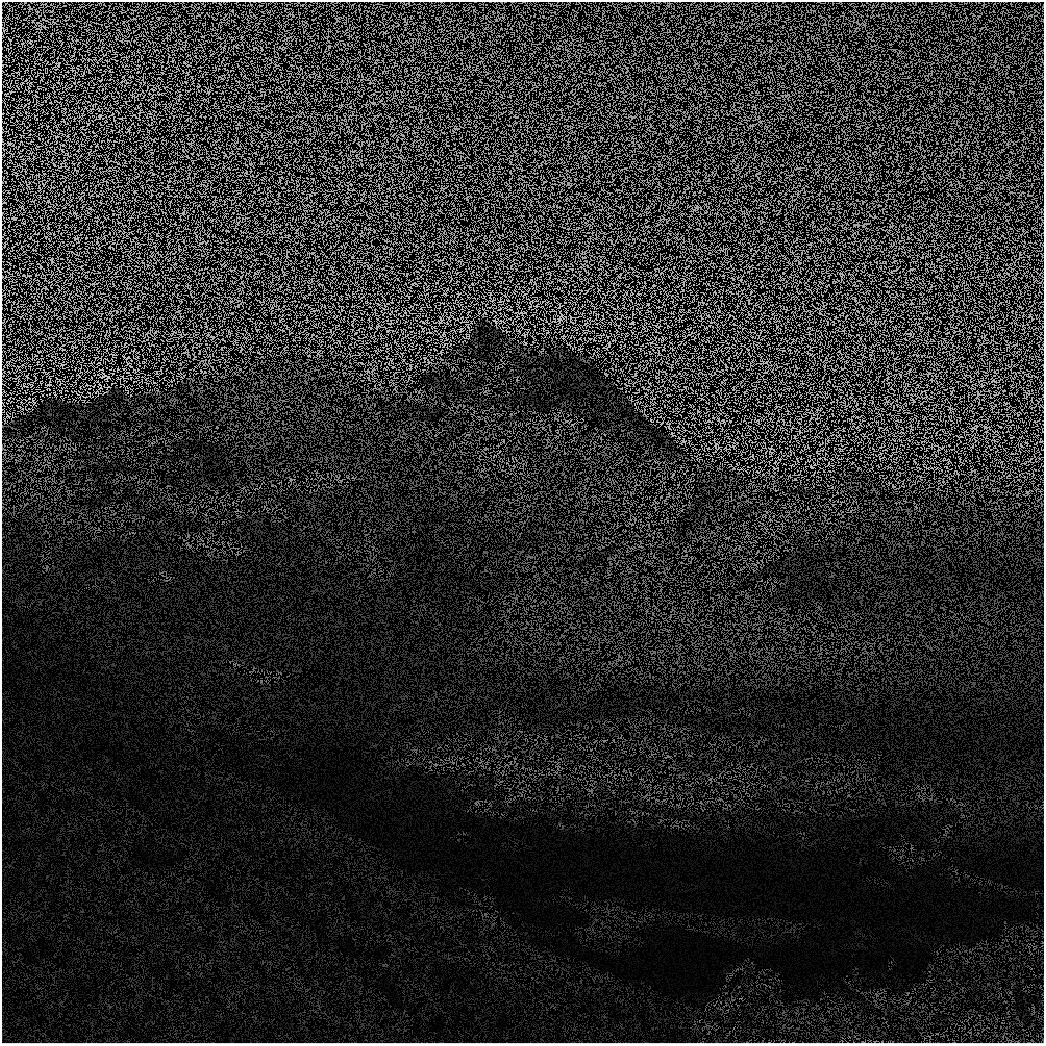
\includegraphics[width=\linewidth]{\mapa/slikaInput35.png}
        \caption{Slika z $35\%$ znanimi podatki.}
    \end{subfigure}
    \begin{subfigure}{0.49\linewidth}
        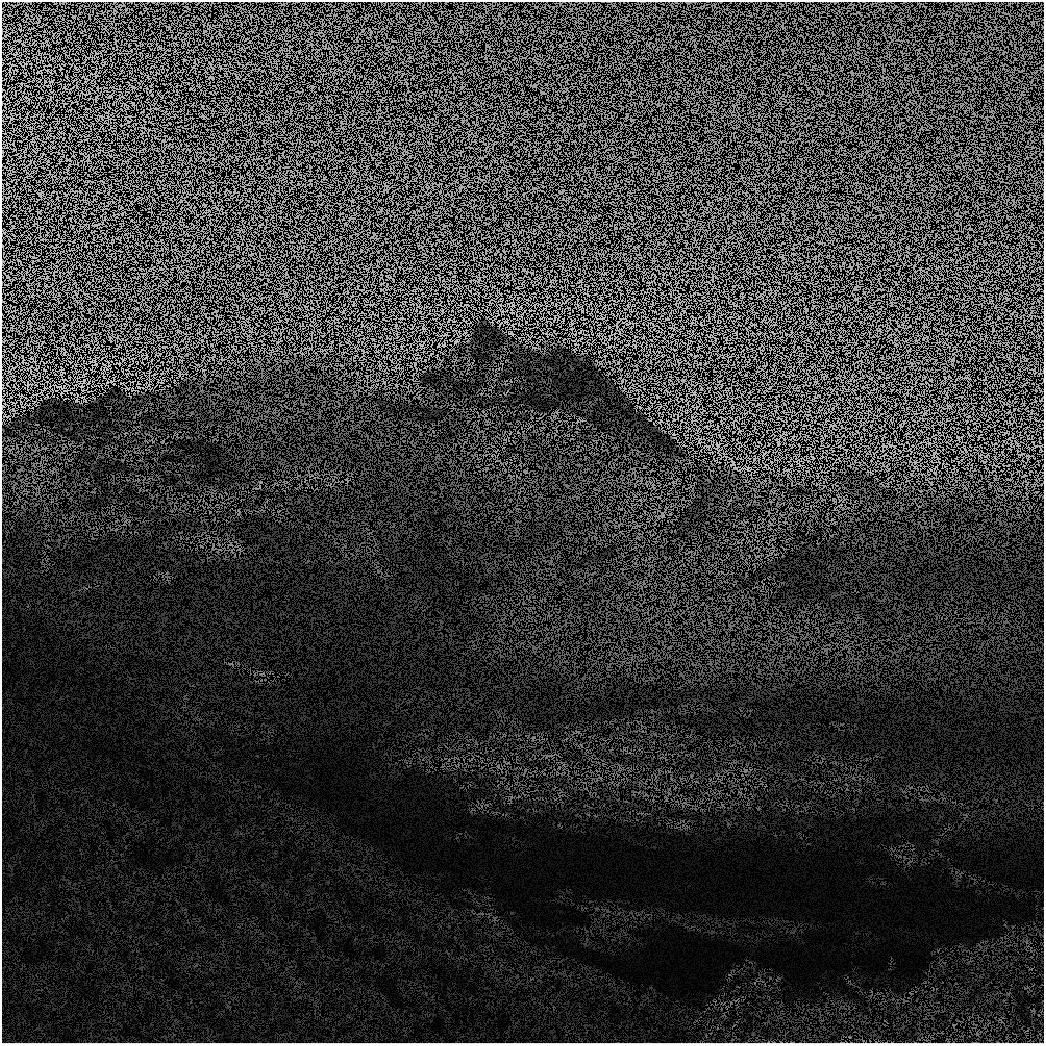
\includegraphics[width=\linewidth]{\mapa/slikaInput45.png}
        \caption{Slika z $45\%$ znanimi podatki.}
    \end{subfigure}
    \hfill
    \begin{subfigure}{0.49\linewidth}
        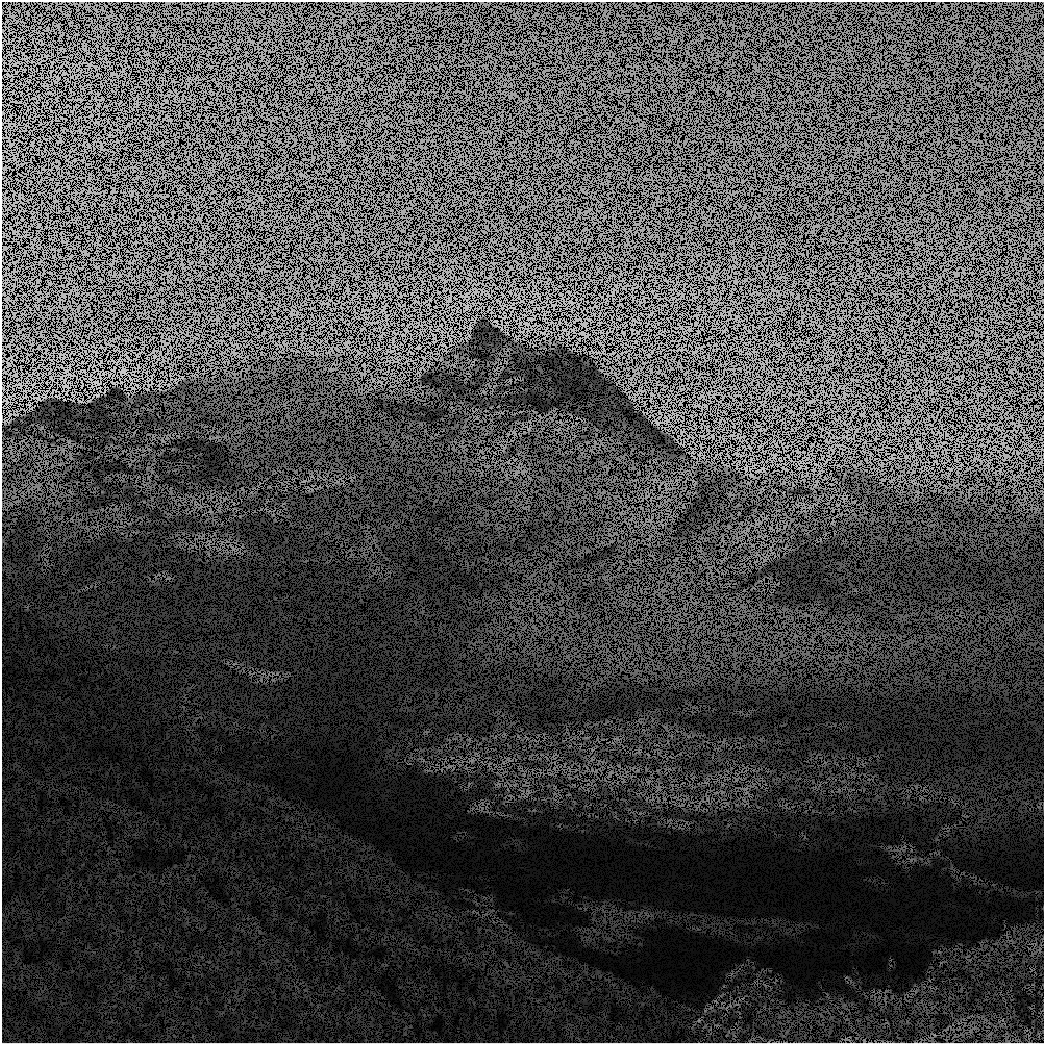
\includegraphics[width=\linewidth]{\mapa/slikaInput60.png}
        \caption{Slika z $60\%$ znanimi podatki.}
    \end{subfigure}
    \caption{Slika uporabljena za rekonstrukcijo. \cite{UnsplashGora}}
\end{figure}

\begin{figure}[!ht]
    \centering
    \begin{subfigure}{0.325\linewidth}
        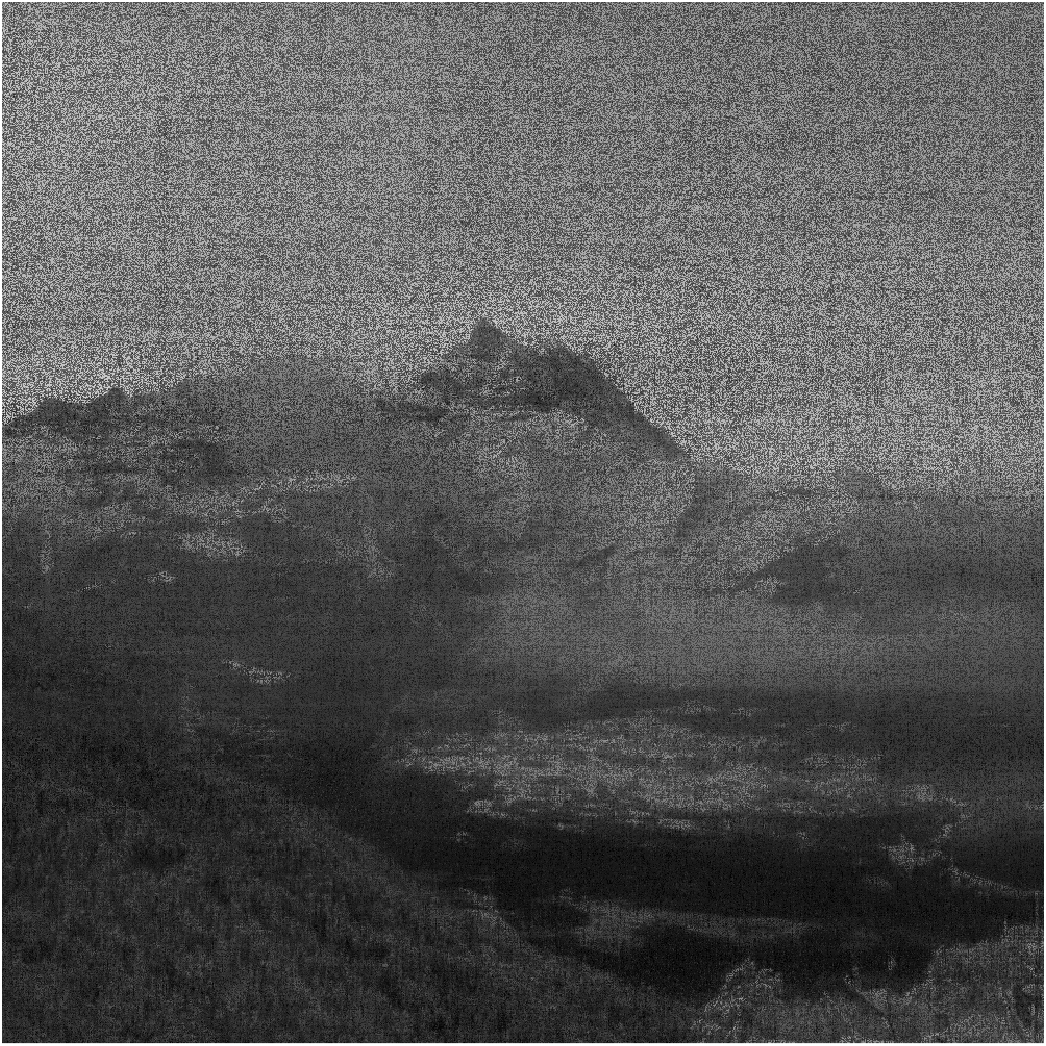
\includegraphics[width=\linewidth]{\mapa/slikaRez35SVT.png}
        \caption{SVT $35\%$}
    \end{subfigure}
    \hfill
    \begin{subfigure}{0.325\linewidth}
        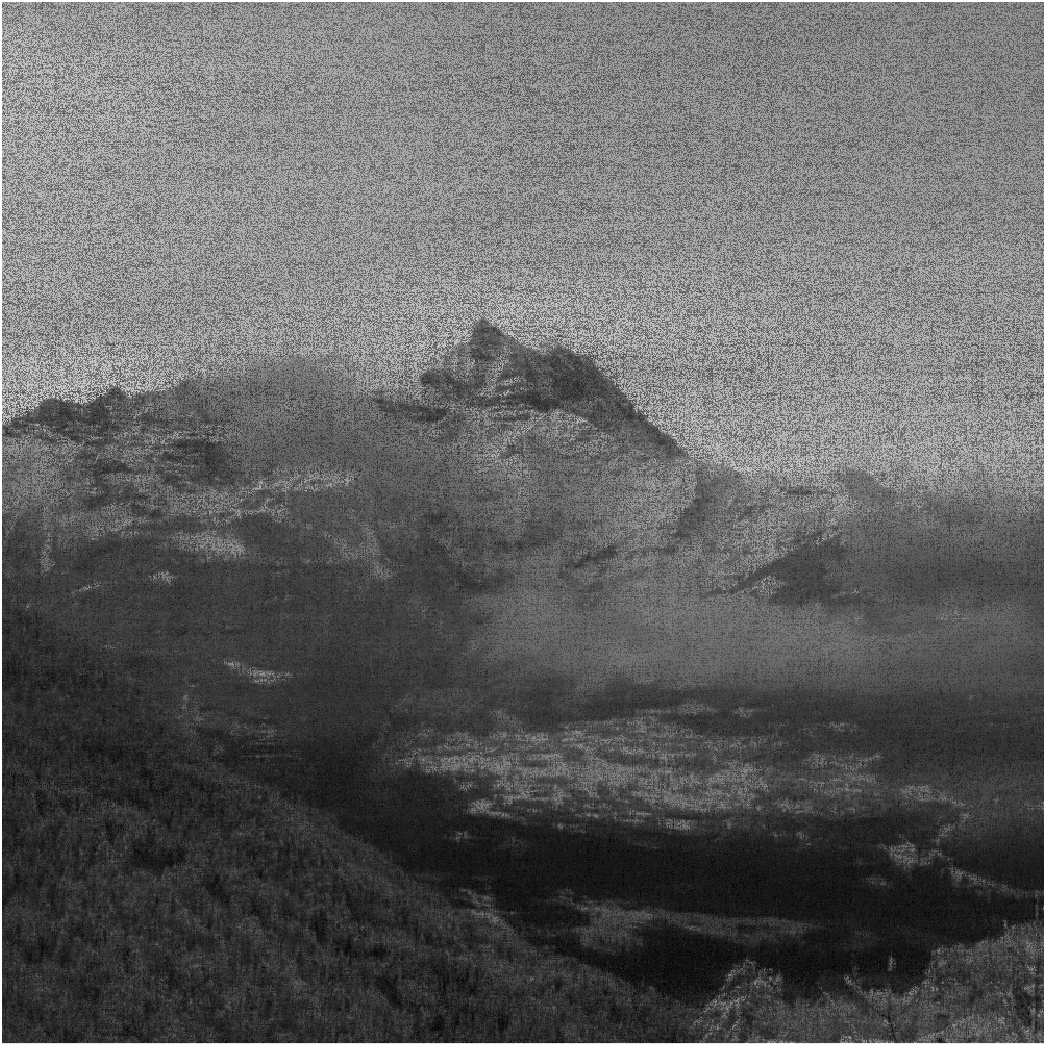
\includegraphics[width=\linewidth]{\mapa/slikaRez45SVT.png}
        \caption{SVT $45\%$}
    \end{subfigure}
    \hfill
    \begin{subfigure}{0.325\linewidth}
        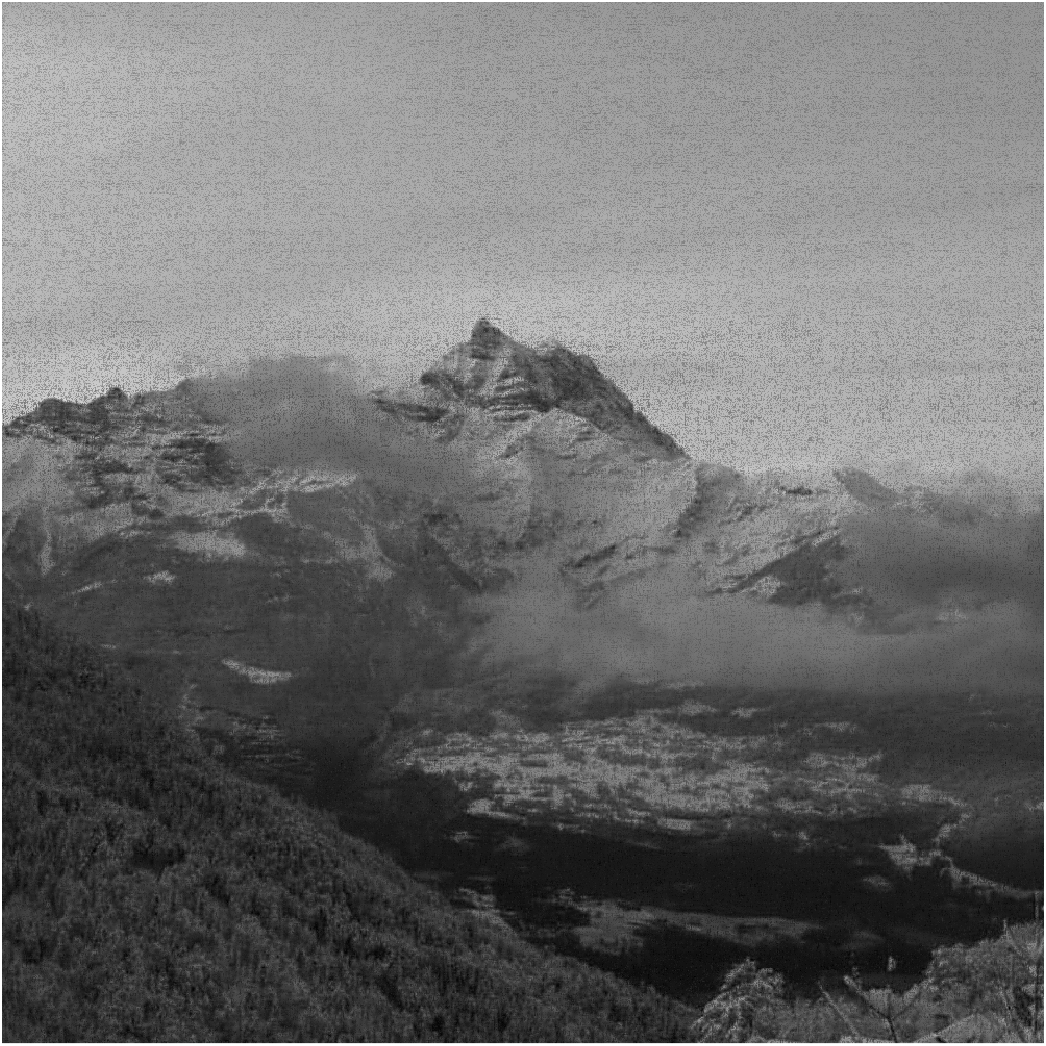
\includegraphics[width=\linewidth]{\mapa/slikaRez60SVT.png}
        \caption{SVT $60\%$}
    \end{subfigure}
    \begin{subfigure}{0.325\linewidth}
        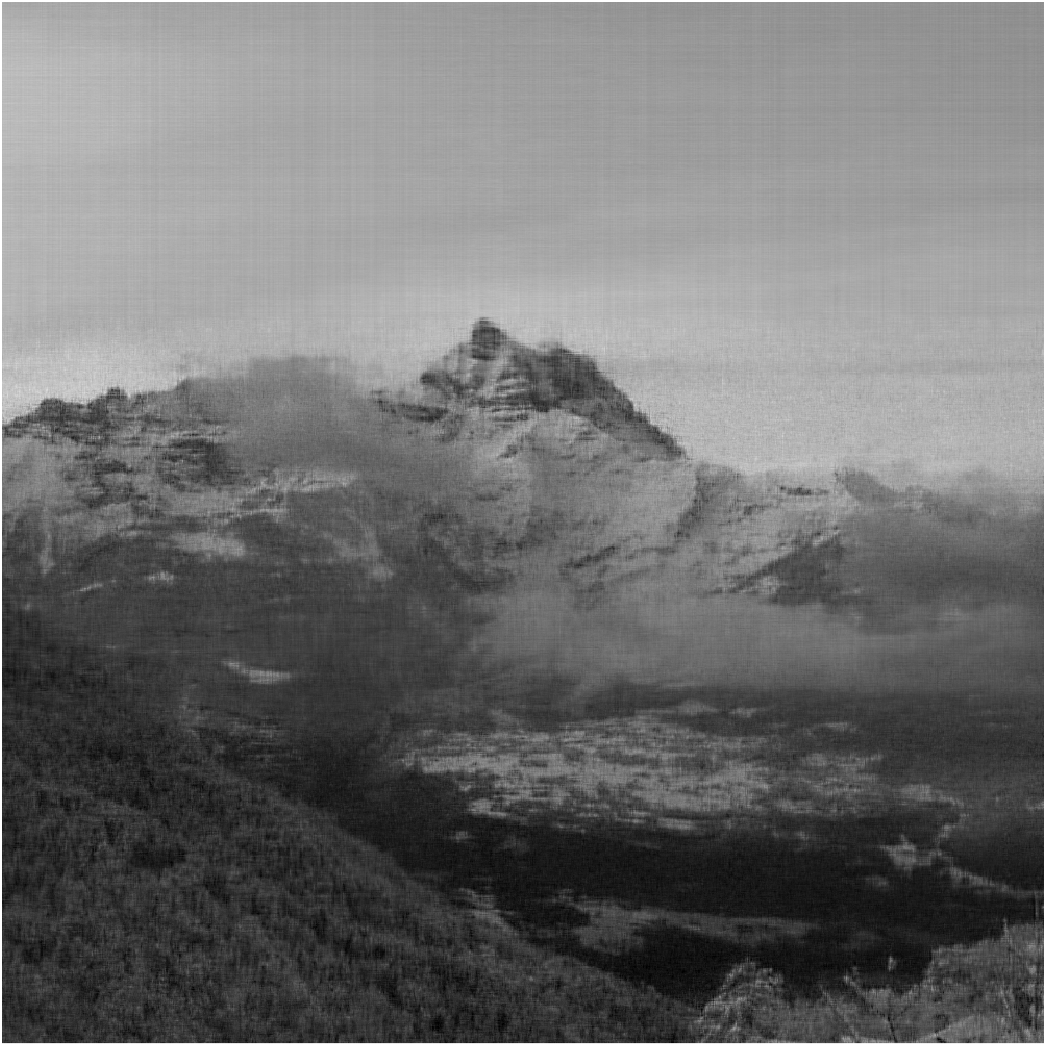
\includegraphics[width=\linewidth]{\mapa/slikaRez35TNNM.png}
        \caption{TNNM $35\%$}
    \end{subfigure}
    \hfill
    \begin{subfigure}{0.325\linewidth}
        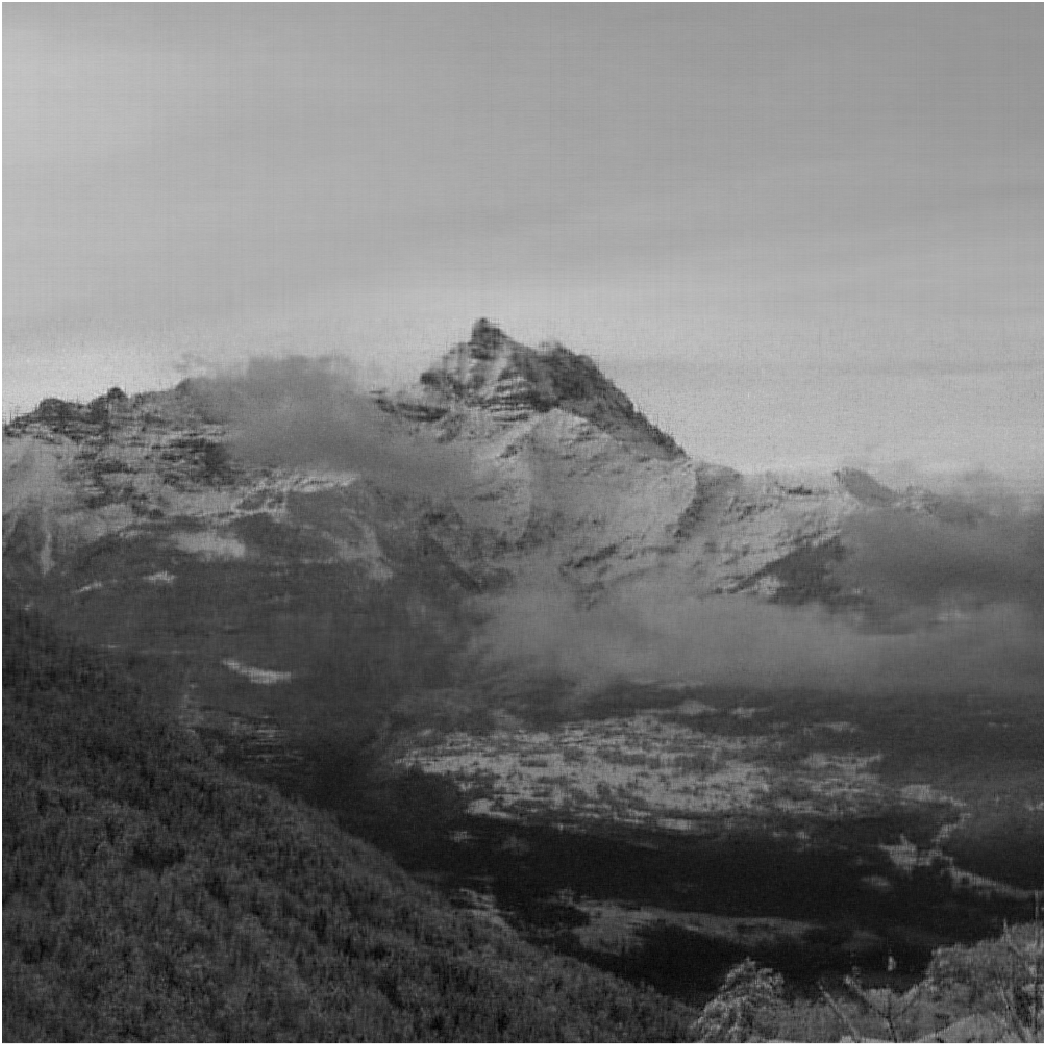
\includegraphics[width=\linewidth]{\mapa/slikaRez45TNNM.png}
        \caption{TNNM $45\%$}
    \end{subfigure}
    \hfill
    \begin{subfigure}{0.325\linewidth}
        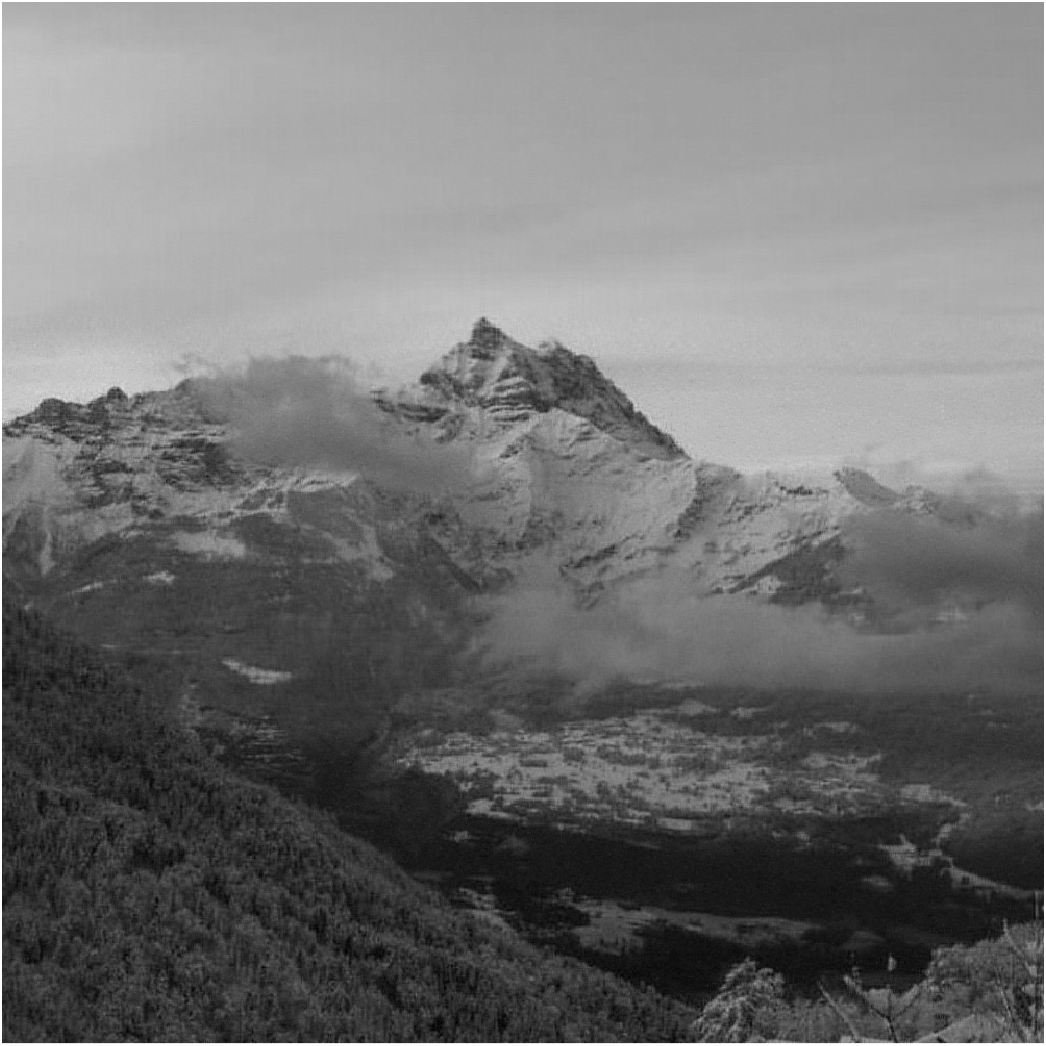
\includegraphics[width=\linewidth]{\mapa/slikaRez60TNNM.png}
        \caption{TNNM $60\%$}
    \end{subfigure}
    \begin{subfigure}{0.325\linewidth}
        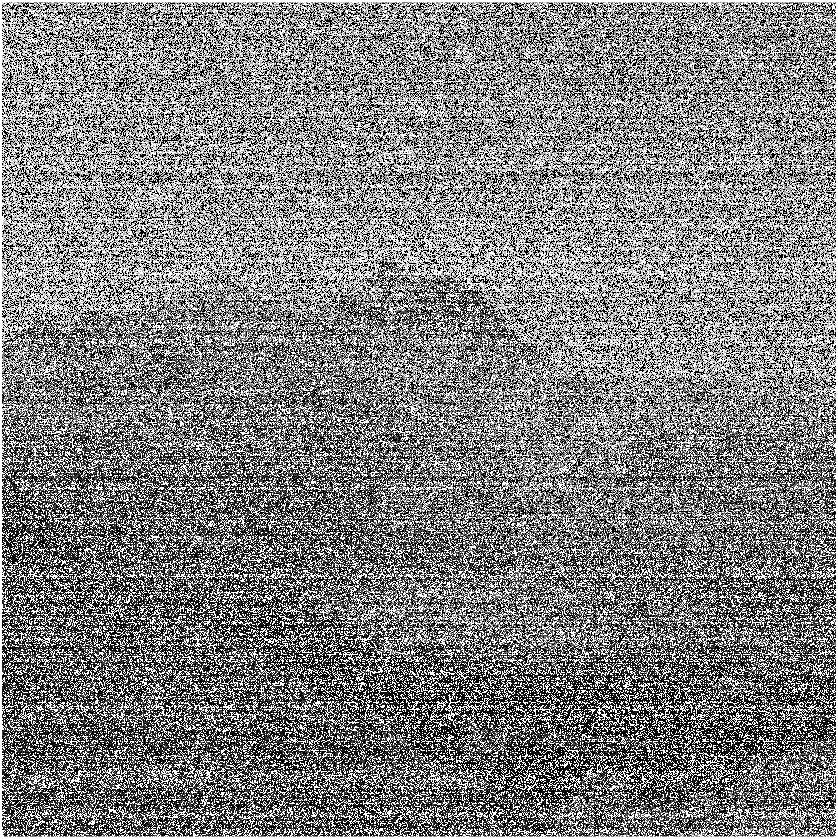
\includegraphics[width=\linewidth]{\mapa/slikaRez35ASD400.png}
        \caption{ASD $35\%$}
    \end{subfigure}
    \hfill
    \begin{subfigure}{0.325\linewidth}
        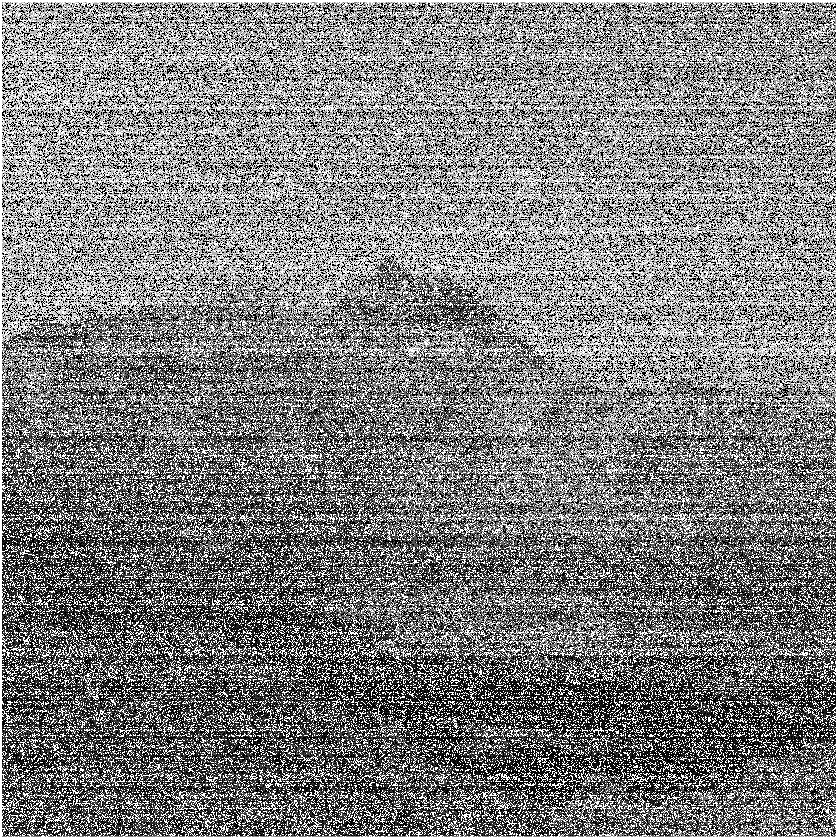
\includegraphics[width=\linewidth]{\mapa/slikaRez45ASD600.png}
        \caption{ASD $45\%$}
    \end{subfigure}
    \begin{subfigure}{0.325\linewidth}
        %ASD 60?%
        \hfill
    \end{subfigure}
    \begin{subfigure}{0.325\linewidth}
        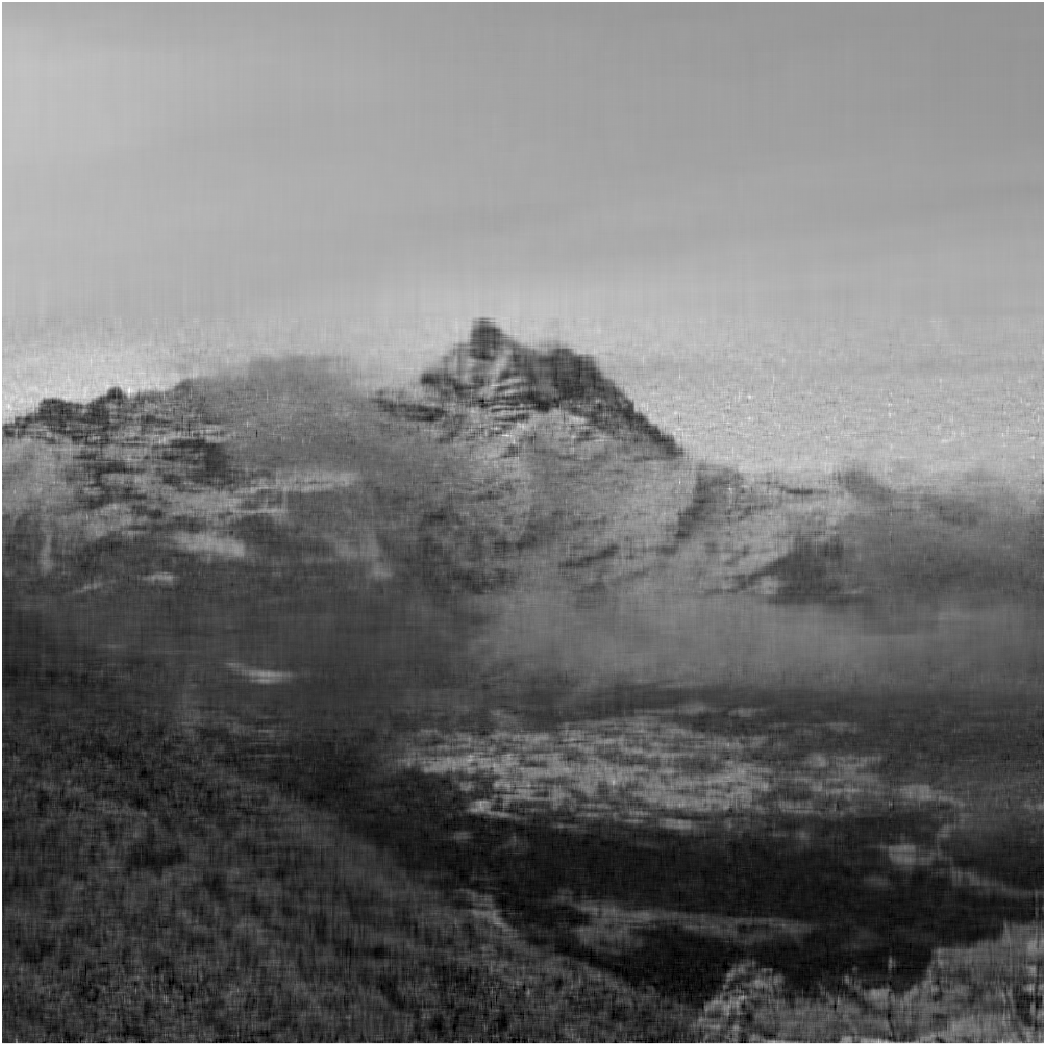
\includegraphics[width=\linewidth]{\mapa/slikaRez35LmaFIT50.png}
        \caption{LMaFit $35\%$}
    \end{subfigure}
    \hfill
    \begin{subfigure}{0.325\linewidth}
        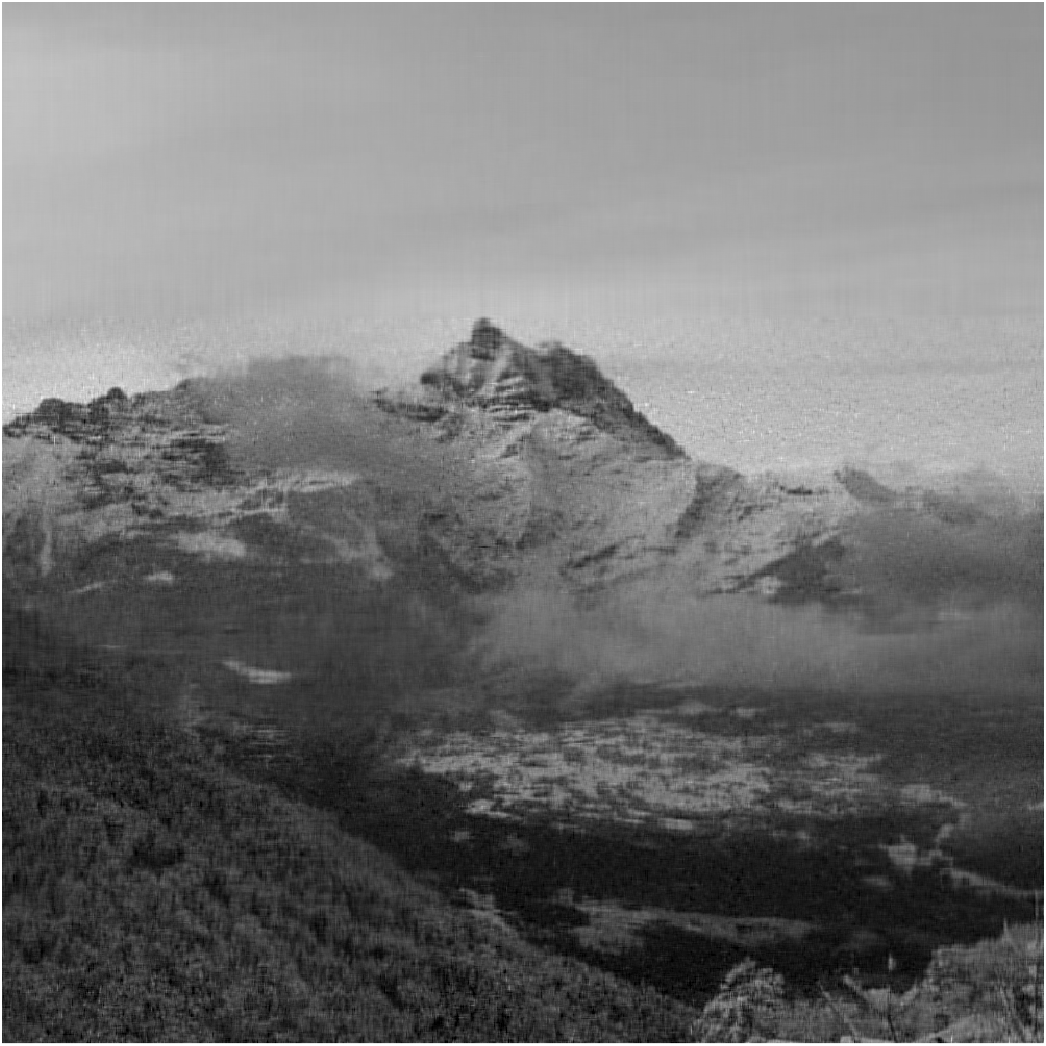
\includegraphics[width=\linewidth]{\mapa/slikaRez45LmaFIT73.png}
        \caption{LMaFit $45\%$}
    \end{subfigure}
    \begin{subfigure}{0.325\linewidth}
        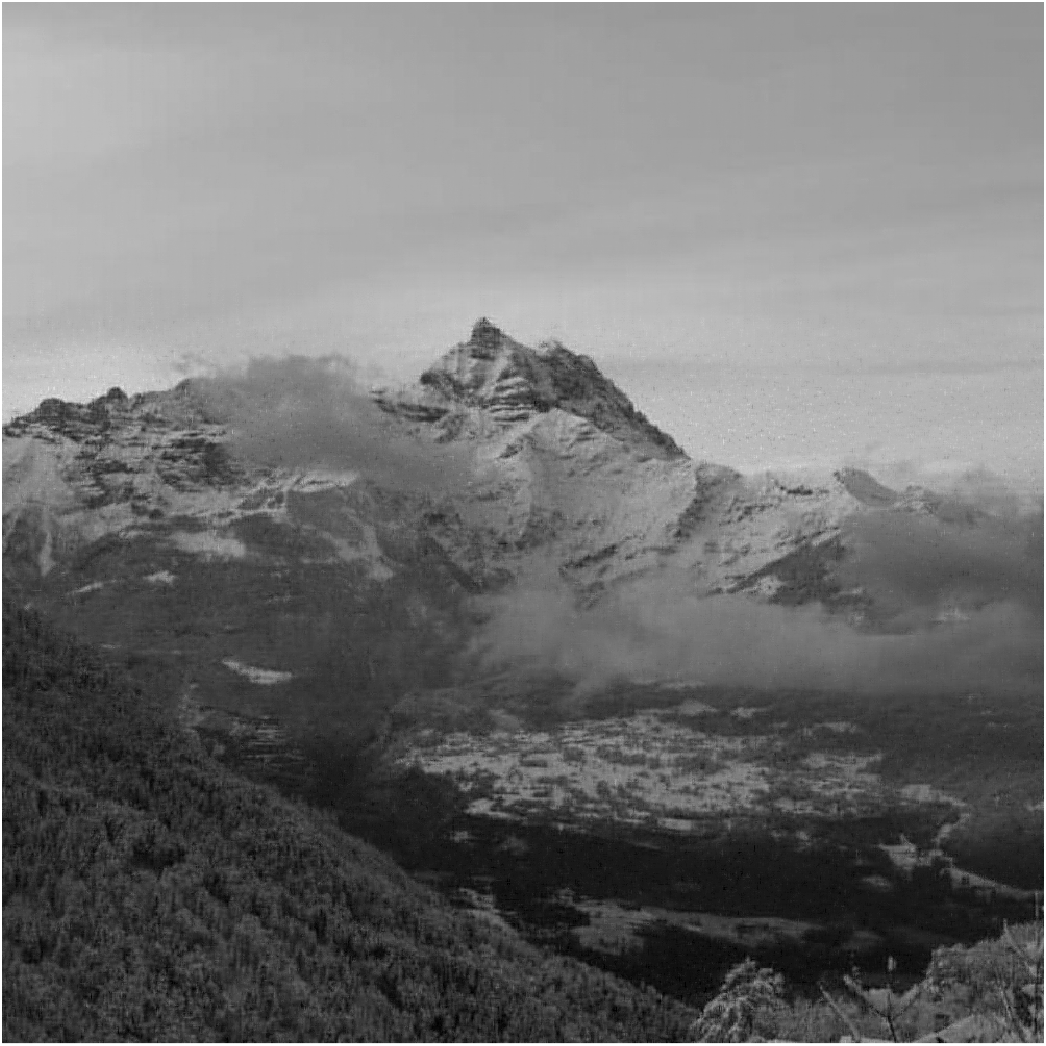
\includegraphics[width=\linewidth]{\mapa/slikaRez60LmaFIT77.png}
        \caption{LMaFit $60\%$}
    \end{subfigure}
\end{figure}
\FloatBarrier

Kot vidimo, je med rezultati velika razlika. Očitno je, da algoritmi TNNM, SVT in LMaFit delujejo najbolje, medtem ko ima algoritem ADDM vprašljive rezultate. Te si lahko interpretiramo kot posledico lastnosti, da lahko algoritem končata v lokalnem minimumu. Prav tako algoritem ADMM ni našel rešitve, ko je imel poznanih $0.60$ podatkov. Zato je ta algoritma smiselno uporabljati, kadar imamo dober začeten približek matrik $X$ in $Y$ ter manj poznanih vrednosti. Algoritem NNM smo med rezultati izpustili, saj je zaradi velikega števila matrik, potrebnih za definicijo omejitev, algoritem preveč prostorsko kompleksen. Ta algoritem bomo zato obravnavali posebej. Zaradi teh opazk se v naslednjih podpoglavjih v večini osredotočamo na algoritme SVT, TNNM in LMaFit.
\todo{je potrebno in graf in tabelo?}
\begin{table}[h]
    \centering
    \begin{tabular}{|c|c|c|c|c|}
    \hline
    & SVT & TNNM & LMAFIT & ASD \\ \hline
    0.35 & $4.69 \times 10^4$ & $7.70 \times 10^3$ & $8.03 \times 10^3$ & $3.9743 \times 10^7$ \\ \hline
    0.45 & $3.15 \times 10^4$ & $5.30 \times 10^3$ & $6.40 \times 10^3$ & $6.0910 \times 10^7$ \\ \hline
    0.6 & $1.25 \times 10^4$ & $3.58 \times 10^3$ & $5.35 \times 10^3$ & - \\ \hline
    \end{tabular}
\end{table}
\begin{figure}[!ht]
    \centering
    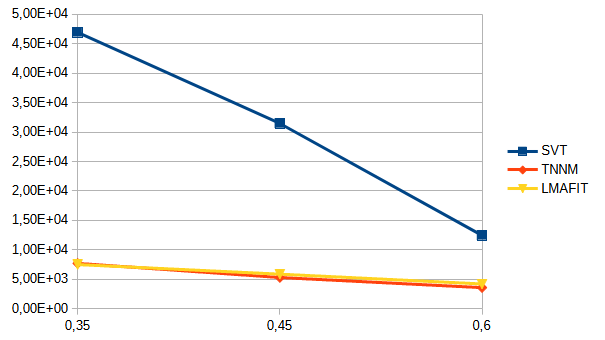
\includegraphics[width=\linewidth]{Poglavja/Slike/grayscale1000/grafNapake.png}
    \caption{Napake algoritmov glede na delež znanih vrednosti}
\end{figure}

\begin{table}[h]
    \centering
    \begin{tabular}{|c|c|c|c|c|}
    \hline
    & SVT & TNNM & LMAFIT & ASD \\ \hline
    0.35 & 338s & 824s & 235s & 1012s \\ \hline
    0.45 & 510s & 498s & 342s & 328s\\ \hline
    0.6 & 1674s & 350s & 48s & - \\ \hline
    \end{tabular}
\end{table}
\begin{figure}[!ht]
    \centering
    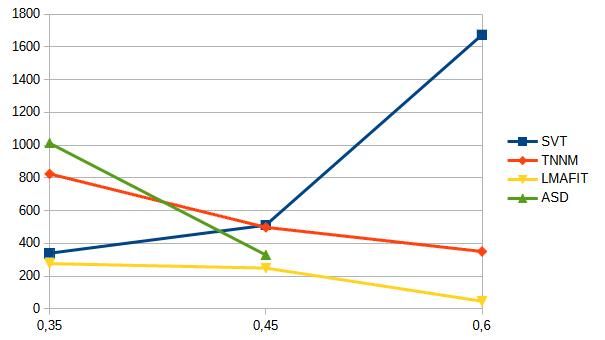
\includegraphics[width=\linewidth]{Poglavja/Slike/grayscale1000/grafCas.png}
    \caption{Časi izvajanja algoritmov glede na delež znanih vrednosti}
\end{figure}

\section{Vpliv kompleksnosti slik na napolnjevanje}
Eno izmed glavnih vprašanj, ki se nam lahko porodi pri implementaciji algoritmov za napolnitev matrik je, kako sama kompleksnost slik vpliva na točnost rezultatov. Ker slike naključnih vrednosti ni mogoče rekonstruirati, lahko sklepamo, da bodo slike s preprostimi motivi napolnjene bolje. Za namene testiranja je torej smiselno izbrati tako preprosto kot tudi vizualno nasičeno sliko. V naših testiranjih uporabljamo sliki knjige in mesta. Sliki sta velikosti $300 \times 300$ pikslov
\renewcommand{\mapa}{Poglavja/Slike/kompleksnost}

\begin{figure}[!ht]
    \begin{subfigure}{0.5\linewidth}
        
\includegraphics[width=\linewidth]{\mapa/preprosta grayscale 300/knjiga.png}
        \caption{Slika s preprostim motivom.}
    \end{subfigure}
    \hfill
    \begin{subfigure}{0.5\linewidth}
        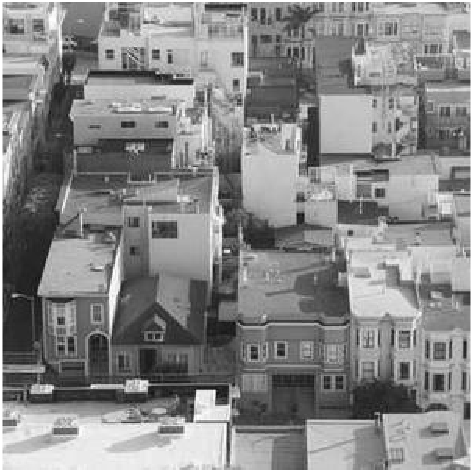
\includegraphics[width=\linewidth]{\mapa/kompleksna grayscale 300/mesto.png}
        \caption{Slika s kompleksnim motivom.}
    \end{subfigure}
    \caption{Vira slik: \cite{UnsplashKnjiga,UnsplashMesto}.}
\end{figure}

\begin{figure}[!ht]
    \begin{subfigure}{0.325\linewidth}
        \includegraphics[width=\linewidth]{\mapa/preprosta grayscale 300/rez35SVT.png}
    \end{subfigure}
    \hfill
    \begin{subfigure}{0.325\linewidth}
        \includegraphics[width=\linewidth]{\mapa/preprosta grayscale 300/rez45SVT.png}
    \end{subfigure}
    \hfill
    \begin{subfigure}{0.325\linewidth}
        \includegraphics[width=\linewidth]{\mapa/preprosta grayscale 300/rez60SVT.png}
    \end{subfigure}
    \caption{Rekonstrukcija preprostega motiva z algoritmom SVT. Odstotki znanih vrednosti slik so bili 35\% (leva), 45\% (sredinska) in 60\% (desna).
    }
\end{figure}
    
\begin{figure}[!ht]
    \begin{subfigure}{0.325\linewidth}
        \includegraphics[width=\linewidth]{\mapa/kompleksna grayscale 300/rez35SVT.png}
    \end{subfigure}
    \hfill
    \begin{subfigure}{0.325\linewidth}
        \includegraphics[width=\linewidth]{\mapa/kompleksna grayscale 300/rez45SVT.png}
    \end{subfigure}
    \hfill
    \begin{subfigure}{0.325\linewidth}
        \includegraphics[width=\linewidth]{\mapa/kompleksna grayscale 300/rez60SVT.png}
    \end{subfigure}
    \caption{Rekonstrukcija kompleksnega motiva z algoritmom SVT. Odstotki znanih vrednosti slik so bili 35\% (leva), 45\% (sredinska) in 60\% (desna).}
\end{figure}

\begin{figure}[!ht]
    \begin{subfigure}{0.325\linewidth}
        \includegraphics[width=\linewidth]{\mapa/preprosta grayscale 300/rez35TNNM.png}
    \end{subfigure}
    \hfill
    \begin{subfigure}{0.325\linewidth}
        
\includegraphics[width=\linewidth]{\mapa/preprosta grayscale 300/rez45TNNM.png}
    \end{subfigure}
    \hfill
    \begin{subfigure}{0.325\linewidth}
        \includegraphics[width=\linewidth]{\mapa/preprosta grayscale 300/rez60TNNM.png}
    \end{subfigure}
    \caption{Rekonstrukcija preprostega motiva z algoritmom TNNM. Odstotki znanih vrednosti slik so bili 35\% (leva), 45\% (sredinska) in 60\% (desna).}
\end{figure}

\begin{figure}[!ht]
    \begin{subfigure}{0.325\linewidth}
        \includegraphics[width=\linewidth]{\mapa/kompleksna grayscale 300/rez35TNNM.png}
    \end{subfigure}
    \hfill
    \begin{subfigure}{0.325\linewidth}
        
\includegraphics[width=\linewidth]{\mapa/kompleksna grayscale 300/rez45TNNM.png}
    \end{subfigure}
    \hfill
    \begin{subfigure}{0.325\linewidth}
        \includegraphics[width=\linewidth]{\mapa/kompleksna grayscale 300/rez60TNNM.png}
    \end{subfigure}
    \caption{Rekonstrukcija kompleksnega motiva z algoritmom TNNM. Odstotki znanih vrednosti slik so bili 35\% (leva), 45\% (sredinska) in 60\% (desna).}
\end{figure}

\begin{figure}[!ht]
    \begin{subfigure}{0.325\linewidth}
        \includegraphics[width=\linewidth]{\mapa/preprosta grayscale 300/rez35LMaFit.png}
    \end{subfigure}
    \hfill
    \begin{subfigure}{0.325\linewidth}
        \includegraphics[width=\linewidth]{\mapa/preprosta grayscale 300/rez45LMaFit.png}
    \end{subfigure}
    \hfill
    \begin{subfigure}{0.325\linewidth}
        \includegraphics[width=\linewidth]{\mapa/preprosta grayscale 300/rez60LMaFit.png}
    \end{subfigure}
    \caption{Rekonstrukcija preprostega motiva z algoritmom LMaFit. Odstotki znanih vrednosti slik so bili 35\% (leva), 45\% (sredinska) in 60\% (desna).}
\end{figure}

\begin{figure}[!ht]
    \begin{subfigure}{0.325\linewidth}
        \includegraphics[width=\linewidth]{\mapa/kompleksna grayscale 300/rez35LMaFit.png}
    \end{subfigure}
    \hfill
    \begin{subfigure}{0.325\linewidth}
        \includegraphics[width=\linewidth]{\mapa/kompleksna grayscale 300/rez45LMaFit.png}
    \end{subfigure}
    \hfill
    \begin{subfigure}{0.325\linewidth}
        \includegraphics[width=\linewidth]{\mapa/kompleksna grayscale 300/rez60LMaFit.png}
    \end{subfigure}
    \caption{Rekonstrukcija preprostega motiva z algoritmom LMaFit. Odstotki znanih vrednosti slik so bili 35\% (leva), 45\% (sredinska) in 60\% (desna).}
\end{figure}
\todo{Lmafit vcasih potrebno zagnati veckat}
\begin{figure}[!ht]
    \centering
    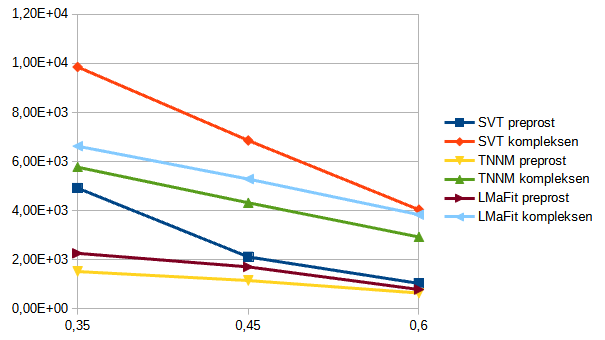
\includegraphics[width=\linewidth]{Poglavja/Slike/kompleksna grayscale 300/kompleksnost.png}
    \caption{Graf napak algoritmov}
\end{figure}

Kot smo pričakovali, so rezultati rekonstrukcije slike s preprostim motivom boljše. Prav tako lahko opazimo, da ima delež znanih vrednosti močnejši vpliv pri sliki s kompleksnim motivom. Napake z dodajanjem informacij torej hitreje padajo pri matrikah večjega ranga. Spomnimo se, da algoritma LMaFit in TNNM za svoje delovanje potrebujeta informacijo o rangu. Pri testiranju je bilo zato potrebno kompleksni sliki podati večjo vrednost ranga, da sta lahko algoritma prišla do dobrih rezultatov.

Sama točnost algoritmov pa ostaja zelo podobna rekonstrukciji velike slike, torej z najboljšimi rezultati pridobljenimi z algoritmom TNNM, nato LMaFit in z najslabšimi rezultati algoritem SVT.

\begin{figure}[!ht]
    \centering
    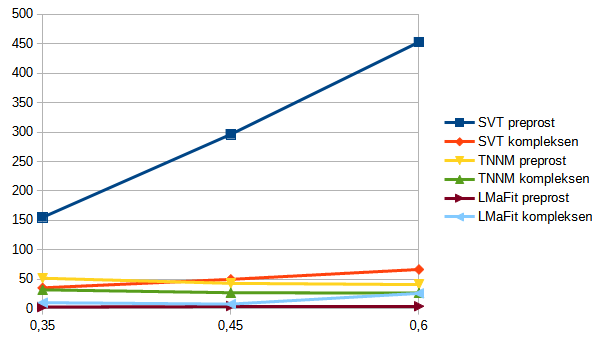
\includegraphics[width=\linewidth]{Poglavja/Slike/kompleksna grayscale 300/cas.png}
    \caption{Graf časov izvajanja algoritmov}
\end{figure}
Sami časi izvajanja pa tu niso tako intuitivni. Prva glavna opazka je, da algoritem SVT potrebuje veliko več časa pri preprostem motivu kot pri kompleksem. \todo{razmisli to interpretacijo} To si lahko razlagamo kot posledico praga. Za dobre rezultate smo pri tako majhni matriki prag nastavili visoko. V našem primeru je imel ta vrednost $3600$. V primeru preprostega motiva, lahko pričakujemo, da bomo imeli malo zelo velikih singularnih vrednosti. Zaradi tega se algoritem težko premika in išče rešitev. Iz tega sledi opazka, da je algoritem SVT bolj smiselno uporabljati za kompleksne motive.

Naslednja pomembna opazka pa je, da delež znanih vrednosti različno vpliva na sam čas izvajanja. Tudi ta faktor je torej lahko pomemben pri izbiri algoritma za reševanje problema. Algoritma SVT in LMaFit potrebujeta za rekonstrukcijo več časa, kadar imata poznanih več vrednosti, medtem ko se algoritmu TNNM z deležem znanih vrednosti čas izvajanja manjša.